\chapter{Deep Learning}

Deep learning is a class of neural network optimization methods for networks that have
 a significant number of hidden layers between their input and output layer.
  Compared to learning algorithms of more simple network structures, the methods of 
  deep learning offer a stable learning success even in the presence of numerous hidden layers.

Deep learning has been successfully applied to object detection in computer vision, in natural language processing,
 and speech recognition. In this chapter we will explain how such artificial neural networks 
 function by looking at feed-forward network as an example. 

\section{Feed-forward neural networks}

A feed-forward network comprises one input layer, H hidden layers and one output layer.
Each layer consists of a number of elements called "neurons". Each neuron of any given layer is 
fully connected to each neuron
of the previous layer. Mathematically, a neural network is represented by a combination of 
matrix multiplication and
activation functions. An activation function determines when a neuron fires.
It usually is nonlinear. The nonlinear characteristic of the activation function is 
what enables the network to learn. Each neuron in a hidden layer can be described by equations \ref{eq:1} and  \ref{eq:2}

\begin{equation} \label{eq:1}
	y_{j} = f(z_{j})
\end{equation}

\begin{equation} \label{eq:2}
z_{j} = \sum w_{ij}*x_{i} + b_{j}
\end{equation}

\begin{figure}[H]
	\centering
	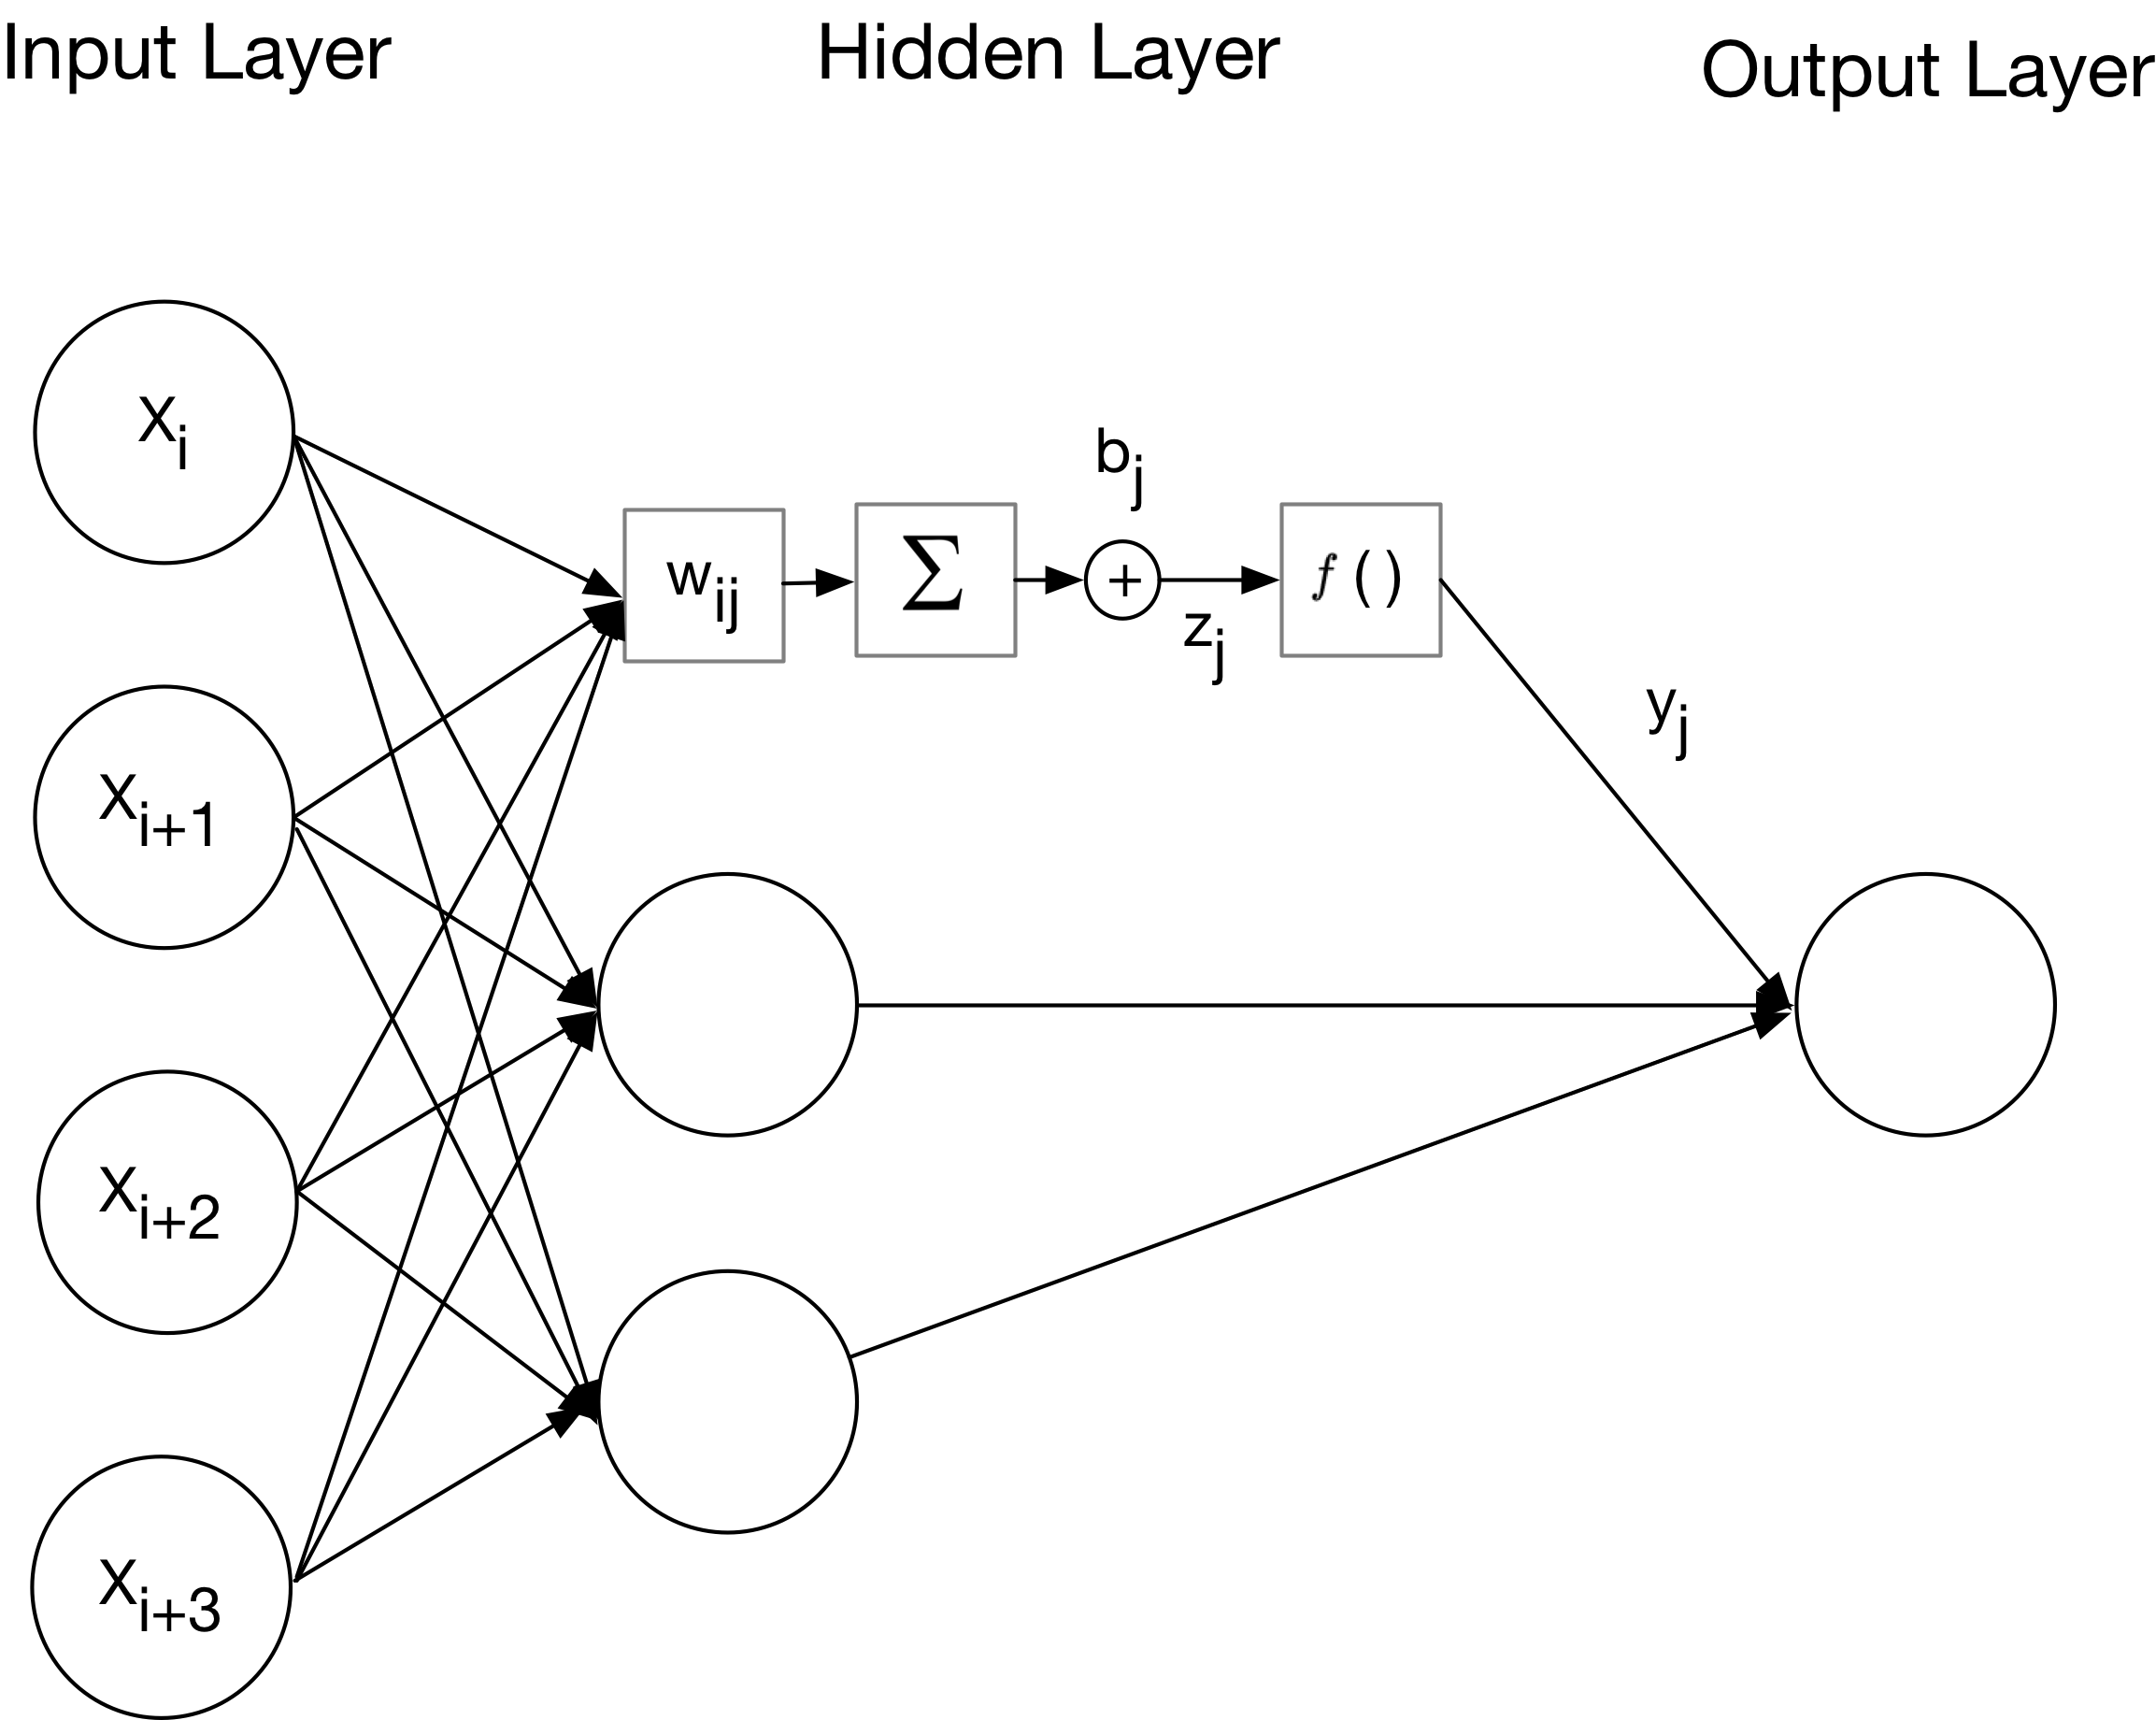
\includegraphics[width=1.0\linewidth]{bilder/grundlagen/fast-forward.png}
	\caption{Schematic view of a  simple two layer fully connected neural network (FCN)}
	\label{fig:FCN}
\end{figure}

The outputs of the preceding layer are each weighted with a weight \(w_{ij}\) before they are accumulated.
The resulting sum is shifted by adding a bias \(b_{j}\) to generate the input \(z_{j}\) for the 
activation function \( f(\cdot) \).
The output of the activation function \(y_{j}\) is then taken as the input for the next 
hidden layer or output layer.
 
 Any continuous functions can be used as activation functions of a neural network. 
 Most common activation functions are sigmoid,  \(f(z) = \dfrac{1}{e^{-z}}\), 
 the hyperbolic tangent, \(f(z) = \frac{exp(z)-exp(-z)}{exp(z)+exp(-z)}\) or the 
 rectifier linear unit (ReLu) \(f(z) = max(0; z)\). ReLu will be used for all future examples.


\begin{figure}[H]
	\centering
	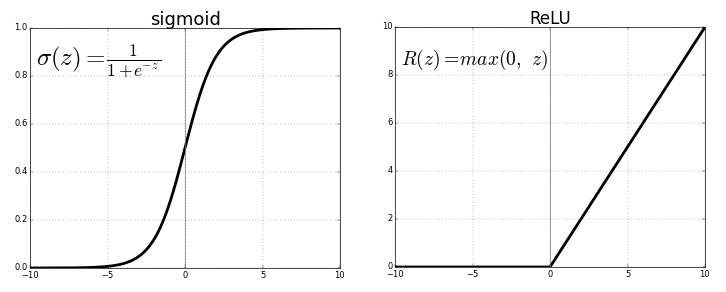
\includegraphics[width=0.8\linewidth]{bilder/grundlagen/sigmoid.png}
	\caption{Sigmoid And ReLu activation function (from\cite{Sigmoid})}
	\label{fig:Sigmoid}
\end{figure}


\subsection{Backpropagation}

Training a neural network means iteratively applying a forward pass followed by an error backpropagation.
During the forward pass the outputs for each neuron are calculated based on its inputs.
The resulting outputs \(y_{out}\) are then compared with the correct answer via a cost function  \(E\).
A common cost function for example is squared error loss (see equation \ref{eq:3}):
 
\begin{equation} \label{eq:3}
	E=\sum\dfrac{1}{2} (target-y_{out}^2) 
\end{equation}

Based on the output of \(E\) it is now possible to check how weights need to be 
adjusted in order to minimize the error.
Applying the chain rule we get equation \ref{eq:4}. 

\begin{equation} \label{eq:4}
	\frac{\partial z}{\partial x} = \frac{\partial z}{\partial y} \frac{\partial y}{\partial x}
\end{equation}

Considering the error  \(E\) we get equation \ref{eq:5}

\begin{equation}  \label{eq:5}
\Delta_{W}E =
\frac{\partial E}{\partial W_{l}} =
\frac{\partial E}{\partial y_{out}}
\frac{\partial y_{out}}{\partial z_{out}}
\frac{\partial z_{out}}{\partial y_{n-1}}
\frac{\partial y_{n-1}}{\partial z_{n-1}}
\end{equation}

Using the calculated gradient $\Delta_{W}E(y_{out})$  it is now possible 
to determine the next weight matrix update using a gradient descent (equation \ref{eq: 6}):

\begin{equation} \label{eq:6}
W_{l}^{t+1}=
W_{l}^{t}-\eta\Delta_{W_{l}^{t}}E(y_{yout)}
\end{equation}

where \(W^{t}\), \(W^{t+1}\) are the current and the updated weight matrices, respectively,
and  \(\eta\) is the learning rate.

\subsection{Weight update}
Calculating the gradient for a complete dataset can take a lot of computation time.
To reduce the amount of computation required
mini-batches can be used to calculate the gradient only based on a few sampled data points. 
Using this analytic gradient a parameter update is performed. There are several ways to perform this update,
the most common one being the stochastic gradient descent (SGD).
In this algorithm, parameters are simply changed along the negative gradient 
direction in order to minimize the error.


\subsection{Initialization}
A neural network needs its weights initialized before it can be trained.
Random initialization is the most common way to create the initial weights.

\subsection{Batch normalization}
To avoid numerical problems due to extreme values the input data is 
normalized (see equation \ref{eq:7}).

\begin{equation}\label{eq:7}
	x \Rightarrow \hat{x} = \dfrac{x-\mu}{\sigma} \Rightarrow x_{norm} = \gamma \hat{x} + \beta
\end{equation}

\(\mu\) and \(\sigma\) are the mean and the  standard deviation of the dataset, respectively. 
\(\gamma\)\ and \(\sigma\) scale and shift the parameters. Batch normalization accelerates 
training time and makes a deep neural network less sensitive to initialization issues.

\section{Classification}
A common task for neural networks is the classification of images, or more general the classification of data into a specific category. The best performing neural network architectures for classifying images are 
convolutional neural networks (CNN). 
All convolutional neural networks consist of convolutional layers followed by pooling 
layers and some fully connected layers.

\subsection{Convolutional layer}
In a convolutional layer several kernels are applied to extract spacial related features. Each output from the the convolutional layer is called a feature-map. Each feature-map was created by a different convolutional kernel of the layer. 

\begin{figure}[H]
	\centering
	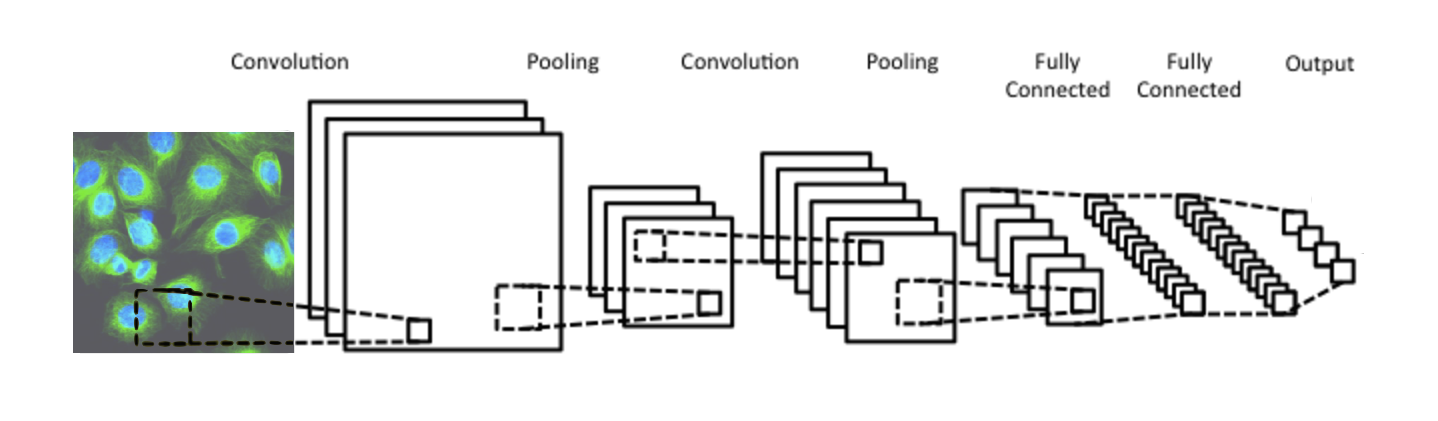
\includegraphics[width=\linewidth]{bilder/grundlagen/convolution.png}
	\caption{Schematic view of a Convolutional Neural Network (CNN) (from \cite{Dao})}
	\label{fig:CNN}
\end{figure}

\subsection{Pooling layer}
After features have been extracted into feature maps,  the pooling layer reduces the 
size of the feature maps and makes them computationally  tractable. A simple implementation 
of a pooling layer is the max-pooling layer, which uses a sliding windows over the input and 
selects the maximum of each window.

\begin{figure}[H]
	\centering
	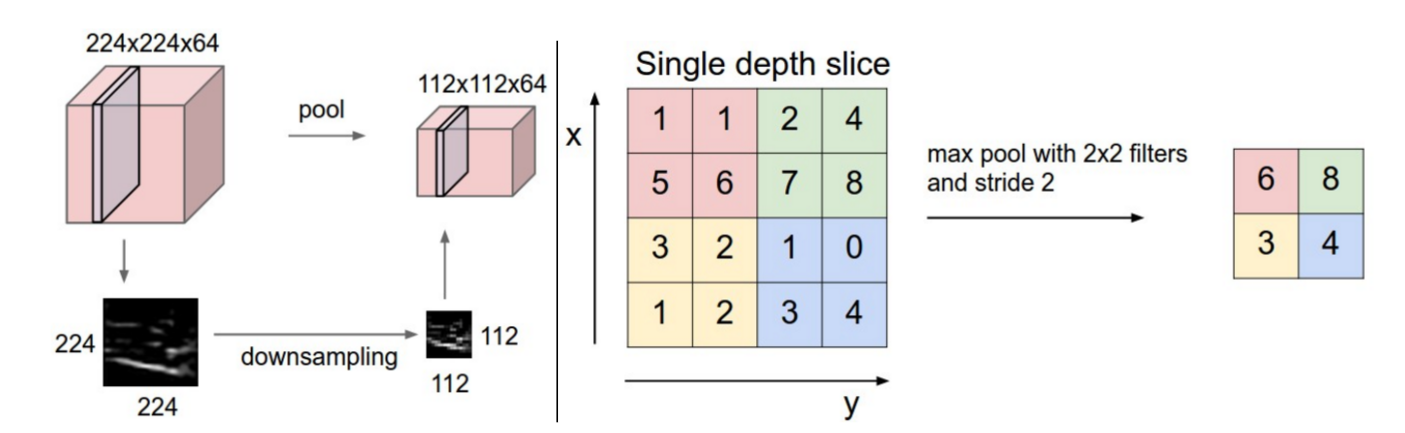
\includegraphics[width=\linewidth]{bilder/grundlagen/pooling.png}
	\caption{Pooling layer (from\cite{Dao})}
	\label{fig:Pooling}
\end{figure}

\subsection{Data augmentation}
Convolutional neural networks need a lot of data to generate satisfactory output. \index{data augmentation}
If not enough data can be provided the data can be artificially augmented by using different approaches.
images can be turned or flipped, cropped, blurred or even resized. This makes it 
possible to generate a lot of data which can be used to further improve training.

\begin{figure}[H]
	\centering
	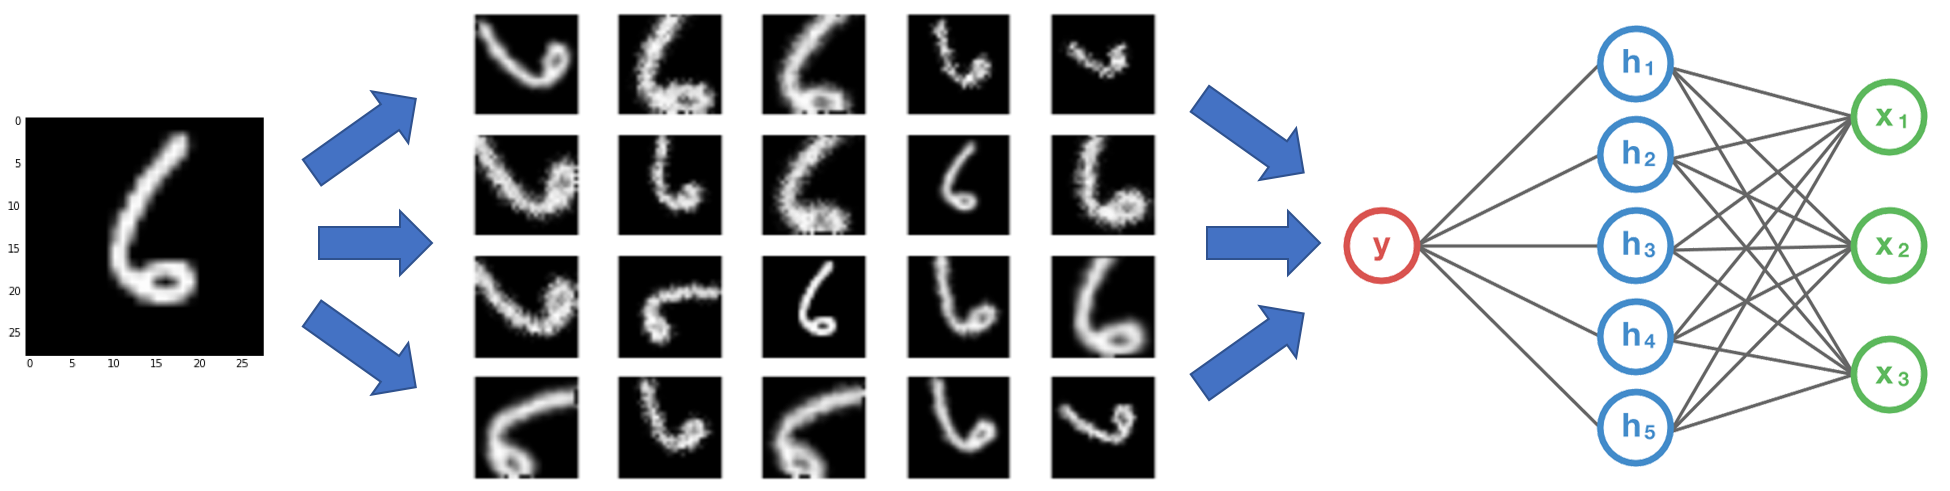
\includegraphics[width=\linewidth]{bilder/deep_learning/data_aug_basic.png}
	\caption{Data augmentation(from  \cite{Ratner2017})}
	\label{fig:COMPONENT}
\end{figure}

